\chapter{Development of Medication Tracking Application}
\label{Kap3}

%talking about platforms in general, to get a common understanding 
\section{Used platforms and technologies} \label{platforms}

This chapter focusses on explaining the used technologies and frameworks for developping the mobile RFID application. In the following, the framework 'Nativescript' which can be used for native mobile development will be explained. After that, a further section will discuss the technology of NoSQL and will compare it to SQL database technology. This section will also depict MongoDB, a document store. Finally, the Impinj RFID reader will be presented. In the last section \pageref{app_development} of this chapter the challenges as well as the user scenarios will be shown. 

\subsection{Native Development with NativeScript} 

There exist several ways to create a mobile application. But the challenge is to develop a consistent solution for the existing systems, like e.g. Android or iOS.
To face the challenge of developing both an Android and iOS application, one has to think of the usage of web development technologies, like for example HTML5, CSS and Javascript. These technologies provide the advantage of using the access to browser/internet  connection.

\subsubsection{NativeScript Sidekick}

\begin{figure}
\centering
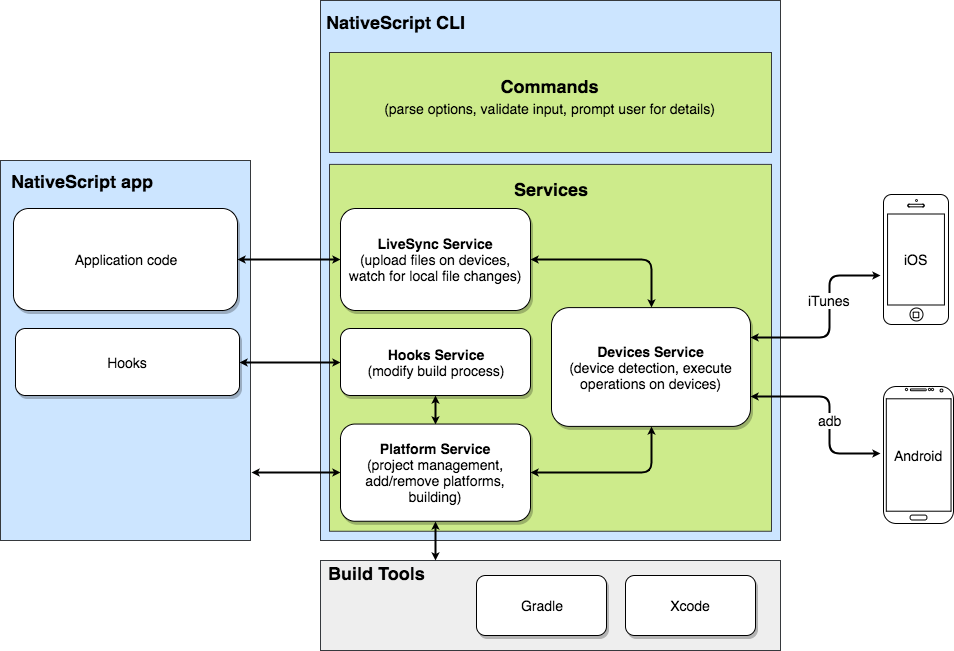
\includegraphics[width=\textwidth]{nativescript_functionality} 
\caption{\label{fig:nsarchitecture}The architecture of NativeScript Applications, adopted from \cite{nsarchitecture}} 
\end{figure}

editor for writing simultaneously apps at one moment (both for Android and iOS devices)

\subsection{Technology of NoSQL} \label{nosql}

There are many possibilities to store data from application systems. \ac{SQL} can be seen as one of the fundamental database technologies used since the 1980/1990ies \cite[p.137 ff.]{nosql_meier}. The technology of SQL offers advantages, such as consistency, security and integrity of data, as well as the protection of transactions. On the other side, there come along many disadvantages while using SQL. To give an example, checking the integrity of data in case of a higher amount of data implicates the need of a higher processing power. Furthermore, facing large-scale development, the efficiency and performance of SQL based systems are decreasing. Moreover, the flexibility and data handling demonstrates another challenge when using SQL. Actually, in practice, the performance is often more important than the consistency, e.g. in social media.    

In addition to that, many companies are missing clear concepts of architecture as well as migration strategies for the optimal application of  'post-relational databases'. To make SQL databases more flexible and to solve the above mentioned problems, Meier and Kaufmann discuss 'post-relational databases' \cite[p.187 ff.]{nosql_meier}. These databases provide on the one hand partial extensions to relational database systems, on the other hand they offer complete new concepts and methods. To give an example, Meier and Kaufmann talk about decentral or federated databases which imply that the data is distributed on different locally seperated computers \cite[p.188 ff.]{nosql_meier}. By replicating the whole data pool and fragmenting it into different smaller parts which are distributed on several computers, decentral databases raise the data volume effectively. The fragments are called 'shards' and the concept of fragmentation is called sharding or partitioning \cite[p.188 ff.]{nosql_meier}. By using decentral databases, users only have to consider the logical view of data and not the physical fragments, all operations on the database will be driven by the database system.  
Alongside the decentral databases there are also introduced other 'post-relational databases', such as 'Temporal databases', 'Multi-dimensional databases', 'Object-relational databases', 'Knowledge/deductive databases' and 'Fuzzy databases'.

However, there were some NoSQL database technologies coming up in the past ten years. In 2000, these databases were called 'Web-Scale-Databases' because of the need of data storage systems which should handle with the large amount of data of web services \cite[p.221 ff.]{nosql_meier}.
The term NoSQL can be understood as 'Not only SQL' which signifies extension of the existing SQL functionalities. Some data specialists prefer the context of 'no relational databases' which is controversial because of the use of graph databases which deal with relations between nodes.   
In the next section, some examples for the NoSQL data management will be explained and compared to the usual SQL data management. According to Meier and Kaufmann \cite[p.3 ff.]{nosql_meier}, SQL databases are formed on a relation-based model which contains tables with entries. Furthermore, each entry has attributes which are defined by a validating range. A table is defined by its table name, the attribute's name and an identification key. It can have both a column or row order or none of these. The relational model indicates that every table is a set of random tuples and that the relations between data is realized by using tables. The result of SQL queries are always tables which can be uniquely, minimally identified by their identification or primary key.

In contrast to that, the technology of NoSQL offers more possibilities to store data, like for example in key-value stores, column stores, document stores or graph databases \cite[p.16 ff.]{nosql_meier}. These four types of NoSQL databases are also called 'Core-NoSQL-Models'. Besides, other NoSQL database models like object databases, \ac{XML} databases or grid databases are defined as 'Soft NoSQL Models'. 
To give some examples of the 'Core-NoSQL-Models', their fundamental characteristics will be described in the following. The key-value stores (e.g. Cassandra) provide the simplest way to store data by using an identification key and a list of values. Document stores (like e.g. MongoDB \pageref{mongodb}) store the data in form of structured text data like \ac{JSON} or XML. In contrast to key-value stores, document stores have a pre-defined structure but are schema-free which means that the data structure can be changed over the time. Graph databases (e.g. Neo4J) introduce a new way to store data: It introduces a graph-based model. Each graph consists of nodes and edges which connect the edges and demonstrate their relations. Each node can have concepts and object. Both, nodes and edges have a label and can contain properties. Each property contains an attribute and a value. The query language for graph databases is called 'Cypher' \cite[p.16 ff.]{nosql_meier} which is a declarative language. Users of Neo4J and other graph databases are able to specify their retrieval query by defining nodes and edges. By evaluating all possible paths (or connections between nodes and edges), the database system calculates all requested patterns.   
Generally, NoSQL technologies are popular for their high availability as well as their protection against system failures by using different replication concepts, e.g. 'Consistent Hashing' \cite[p.11 ff.]{nosql_meier}. In addition, NoSQL is characterized by its vertical and horizontal aligned scalability, its weak or non-existent restrictions concerning schemas and data models. Along, NoSQL databases offers simple data replication and easy access through API \cite[p.221 ff.]{nosql_meier}.  

\paragraph{Document Stores}

In the last section, there were introduced some examples of NoSQL databases. This paragraph reveals with the characteristics, advantages and disadvantages of document stores because the deployed database, MongoDB, is a document store. 
Basically, document stores consists of databases, containing collections with documents. Each document can have its own internal structure and is defined by JSON-like files which look like a list of attribute-value-pairs. As a 
On the one hand, like key-value-stores, document stores are schemafree so that users do not have to define a schema for the database. Nevertheless, document stores offer the possibility of structuring the stored data. In addition to that, the structured data will be stored as records which are called documents. Generally, document stored were developed for web services. Thus, they are easily integrable with JavaScript and \ac{HTTP} and easy horizontally scalable. 
On the other hand, as a disadvantage, document stores do not support referential integrity either normalization.
Nevertheless, because of being schemafree, document stores propose high flexibility to store different data (see section Excursus: BIG DATA \pageref{bigdata}). Referring to the flexibility, fragmentation and sharding of an existing data pool can be seen like that. In excess of relations between data, documents do not have any relation to each other but each document contains a closed collection of data in which familiar data can be linked.

\paragraph{Queries (Map and Reduce)}

Document stores are exceptional in that they query in a Map/Reduce procedure which enables the possibility of querying parallel and accelerated. Consecutive, the Map/Reduce procedure will be explained briefly. 
To begin with, the method can be divided into two phases: During the first phase (Map, 'group by'-phase), the data is grouped by criteria. This is realized by a Map-function which asociates for each document an appropriate specific processing by establishing an index (= map) and sending it back. A map can be compared to an associative array with one or multiple key-value-pairs per document.  
After that, in the second phase (Reduce, 'Aggregation'), a Reduce-function (can be compared to SQL statements) returns for each key in the index a row of the Map-Function and aggregates their related values. This second phase is optional.

\paragraph{ACID vs. BASE}

Concerning the topic of transactions in SQL, Meier and Kaufmann \cite[p.136 ff.]{nosql_meier} mention the \ac{ACID} principle. Atomacity means that a transaction is either performed completely or not. Consistency refers to transactions which cause conviction from one state into another. At this point, Meier and Kaufmann declare a transaction as 'an unit to obtain consistency'. Isolation signifies parallelly run transactions which will produce the same results as single-user environments becaue each transaction is run isolated. The Isolation principle includes the protection from unwanted side-effects. When talking about the isolation of transactions, they can be called 'unit of serializability'. The last principle, durability refers to the different states of databases which have to be maintained until the next transaction. In that case, every transaction can be seen as 'unit of recovery'.

The \ac{BASE} principle which refers to NoSQL technologies says that a consistent state in a distributed database system can take place retartedly.

\subsubsection{Characteristics of NoSQL Databases}

A \ac{DBMS} defines a software which describes, stores, queries data independently from an application \cite[p.2 ff.]{nosql_meier}. It consists both of a storing and managing component. The storing component is composed of all data which has to be stored in organizational form and their description. The managing component contains a querying or manipulating language to evaluate data and to change them, such as access control units and an user interface. When it comes to the use of web applications and a heterogeneous data pool in real-time, SQL databases are often not suitable for these problems. In this case, a NoSQL database should be considered. 

\subsubsection{Excursus: BIG DATA} \label{bigdata}

The following section shall only act as additional contextual knowledge paragraph. 
The term 'Big Data' has been emerged during the past 10 years. Due to the enormous data pool, e.g. in social networks or user analysis, which is not easy to manage with usual software tools, new data technologies were needed. As a solution, NoSQL technologies have been arised. Furthermore, Big Data refers to unstructured data which comes from different sources \cite{nosql_meier}. 

\paragraph{Velocity, Variety, Volume}

When talking about Big Data, often there come up three descriptive terms: Velocity, Variety and Volume. Velocity refers to the real-time high-speed evaluation of the upcoming data. Variety means that there are distinct formats of data: structured, semi-structured and unstructured data. The last characteristic of Big Data, volume, deals with the high amount of data \cite{nosql_meier}. 
Calolas et al. refer to challenges like e.g. dealing with tremendious amounts of data, unstructured data (diversity of \ac{OSN}) as well as the complexity to challenge analyzing social networks data \cites{trends_nosql}.

\subsubsection{Use case of NoSQL Databases: 'Socii System'}

To give an example of the use of NoSQL technologies, the next section will focus on explaining a developed system 'Socii'. 'Socii' was developed from Jroge Daniel Calolas, Alda Lopes Gancarski and Pedro Rangel Henriques. In their article 'Online Social Network Analysis Visualization Using Socii' \cite[p.218-228]{trends_nosql}, they describe the several technological challenges they faced during development but also the benefit of this social network analysis and its scientific importance. In short words, 'Socii' is a system which enables the analysis and visualisation of social networks by helping \ac{OSN} users to exploit and understand their own networks through a user friednly interface. During development, Calolas et al. were facing four main principles: simplicity, accessibility, OSN integration and contextual analysis.
One big problem before developing of 'Socii', Calolas et al. mention was the observation of social structures and the analysis of these networks. By establishing 'Socii', the authors Calolas et al. wanted to proprose to fill the gap or struggle that OSN users have in understanding their network. To give an example of these struggles, there were three main topics, Calolas et al. were facing: 'how relationships evolve along the time', 'what role play these friendships within the network' and 'how they can analyze and visualize their networks based on social properties (such as mutual relationships, geographical positions, personal tastes and preferences or hobbies)' \cite{trends_nosql}. 

\paragraph{Structure and flow of data analysis and visualization systems}

When introducing 'Socii' as an social analysis tool, Calolas et al. also talk about several tasks and steps during the process of data analysis and visualization systems. Firstly, data has to be extracted (through APIs, web crawlers and web scrapper. Secondly, data is achieved which requires careful selection of relevant data to store \cite{trends_nosql}. In order to have an efficient system that provides good structure for data analysis, one needs to select the data carefully. In the third step, data is explored by defining of what one user wants to do with the data. Furthermore, during this step, there are two important questions: What are the applications that can be seen for the stored data? How can the system digest and transform data in order to make it useful and interesting for the end user? 
Lastly, in the fourth step, data is visualized which means the kind of presentating or showing the transformed data is chosen by the user. Particularly, the work of the data scientist has a huge impact on the end user. In generals, the data visualization targets a general audience.  
By extension, 'Socii' affirms web availability, OSN's  integration, contextual analysis and being a trade-off for such gains the system performance.

\paragraph{Main functionalities of 'Socii'}

One of the main functionalities of 'Socii' is information extraction and data mining \cite[p.223]{trends_nosql}. These include extracting some user networks form given OSNs by calling web crawler modules which then return the extracted information. After that, an extraction manager sends the extracted data through a simple data mining process in order to data normalized before it is stored in the database (MongoDB). Web crawlers are implemented in Python and the crawling operations are performed using XPath selectors to extract the information that are needed to build the network.
Generally, the main functionalities of 'Socii' amount to OSN contextual netowrk analysis (with relatively low complexity) \cite[p.227]{trends_nosql}. Moreover, 'Socii' intends to integrate data from different OSNs by processing a set of node properties displayed together with the network structure. Roughly, Calolas et al. implemented three features of 'Socii'. To start with, 'configurable, parameterized analysis' enables users to select several metrics upon a given network. Consequently, 'clear, intuitive social graph visualization and interaction' refers to the visual web component of 'Socii' which provides users a set of visual features (coloring, node discovery etc.). Thirdly, 'Socii' offers an 'organized overview upon SNAs and OSN data' which include visual components that aggregate SNAs metrics and OSNs information. Thus, users are able to cross information from both and can derive conclusions from intersecting the information \cite{trends_nosql}. 

\paragraph{Limitations of 'Socii'}

As shown in the last paragraph, 'Socii' offers many features to analyse Big Data especially in social networks. Nevertheless, Calolas et al. depict some limitations and disadvantages which will be explained in the following. 
First of all, there exists a technical and architectural struggle of feeding the system through an extraction pipeline built on top of the web crawlers. This is known and proved by a very slow, limited and error-prone method for data extraction and the authors call it the 'bottleneck' of their built system \cite [p.227]{trends_nosql}. 

\paragraph{Future outlook of 'Socii'}

According to Calolas et al., 'Socii's implementation should be completed to work with other OSN's. Furthermore, it can be extended to perform evaluation and validation of system with users having accounts in several OSNs and several profiles. 

\subsubsection{NoSQL Technology: MongoDB}\label{mongodb}
\subsubsection{Reasons and Advantages of MongoDB}

\cite{mongodb_edward}

strong consistency and atomicity
secondary indexes 
ad hoc queries
querying/indexing/updating similar to relative databases (like SQL/Microsoft Access)

\subsection{Impinj RFID Lector and Antenna}

\subsubsection{General Information}

\subsubsection{Examples}

%
% talking about application, more details
%
\section{Application development} \label{app_development}

\subsection{Challenges during development}

Mongodb integration within nativescript application 
--> with Node JS package installer 
but synchronization with data from Mongodb was difficult

Real-time synchronization of mobile application with MongoDB server was difficult. Firstly, HTTP Request/Response was implemented to connect the mobile device with the RFID reader and the database. But only one device was enabled to connect to the server. Thus, another solution had to be considered. Finally, a Socket.IO connection was implemented to both server and client. Socket.IO enables two-way data synchronization and cannot be compared to HTTP Request/Response. Furthermore, with Socket.IO, it was possible to run the application on various mobile devices without any complication. 

\subsection{Progress of development}

\subsubsection{User Scenario}

screenshots of app

\begin{figure}
\centering
\subfigure[Start page of application]{\label{fig:a}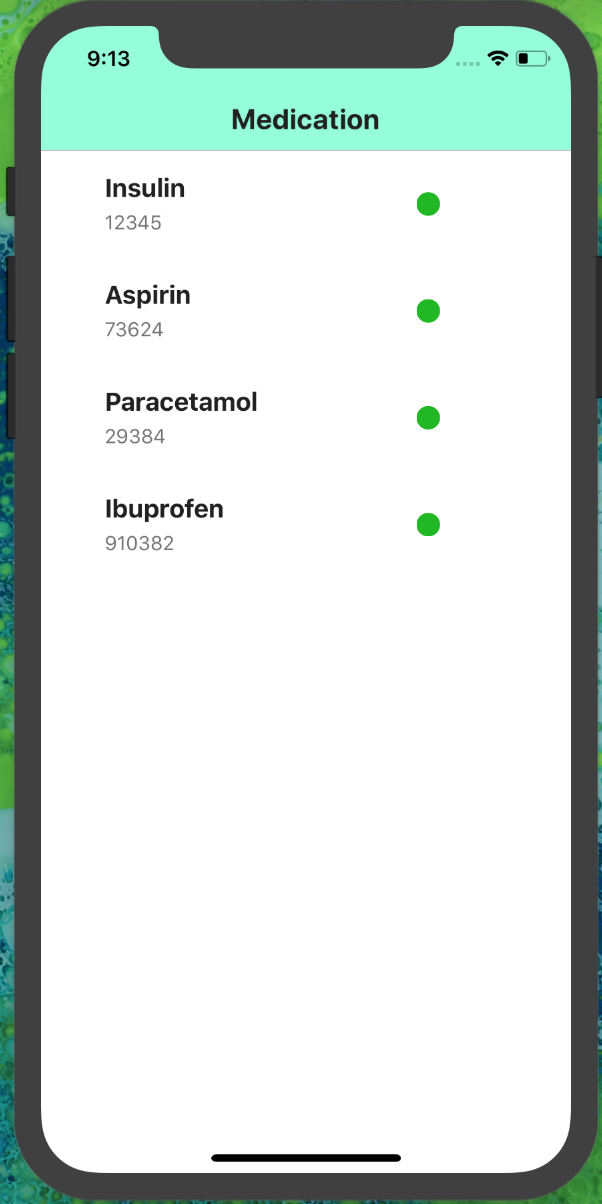
\includegraphics[width=6cm, height=12cm]{Mainview}}
\subfigure[Item information page]{\label{fig:b}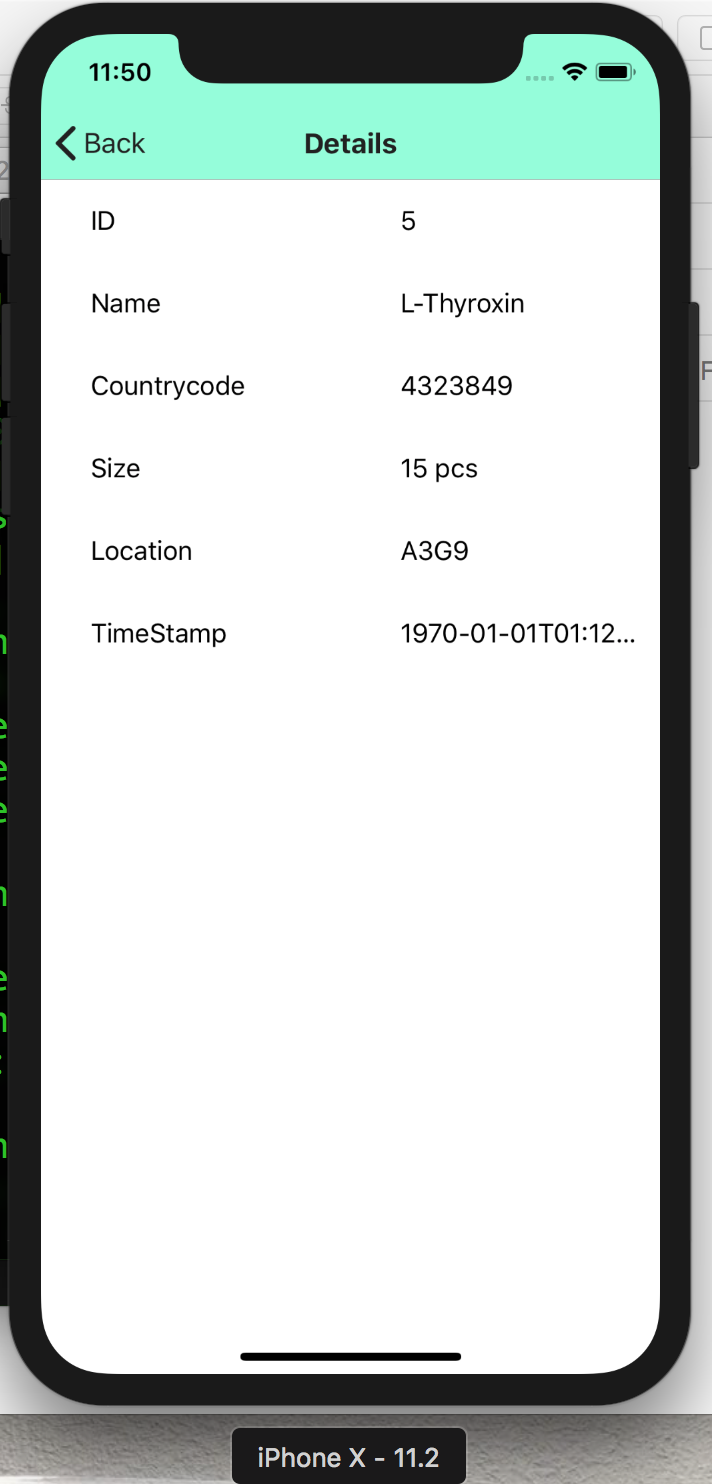
\includegraphics[width=6cm, height=12cm]{Detailview}}
\caption{Layout of application, Screenshot of iOS Simulator}
\end{figure}




\subsubsection{Software Architecture}

\begin{figure}
\centering
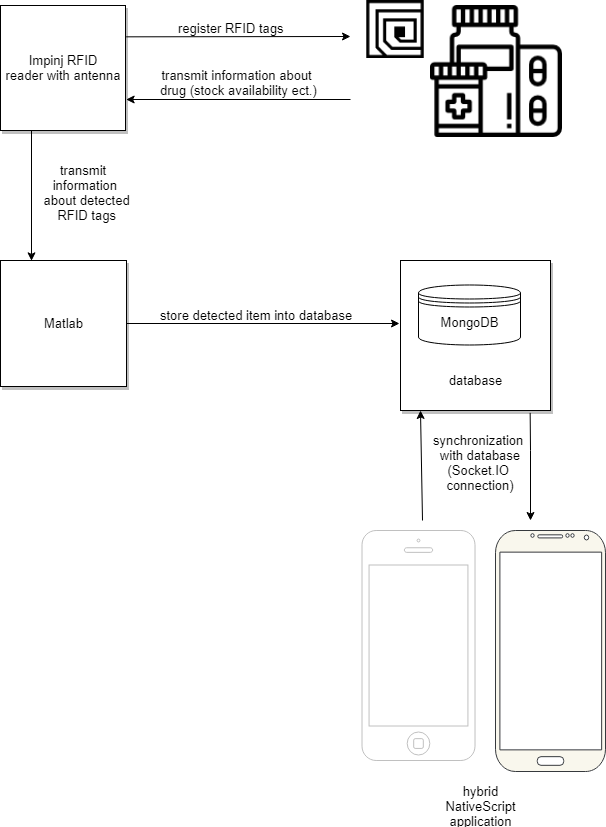
\includegraphics[width=\textwidth]{app_architecture} 
\caption{\label{fig:apparchitecture}The developed system architecture of the mobile RFID application} 
\end{figure}

picture of general software architecture: 
2 antennas, 1 lector (RFID Impinj), Database (MongoDB), GUI: Android and  iOS Application 


\begin{figure}
\centering
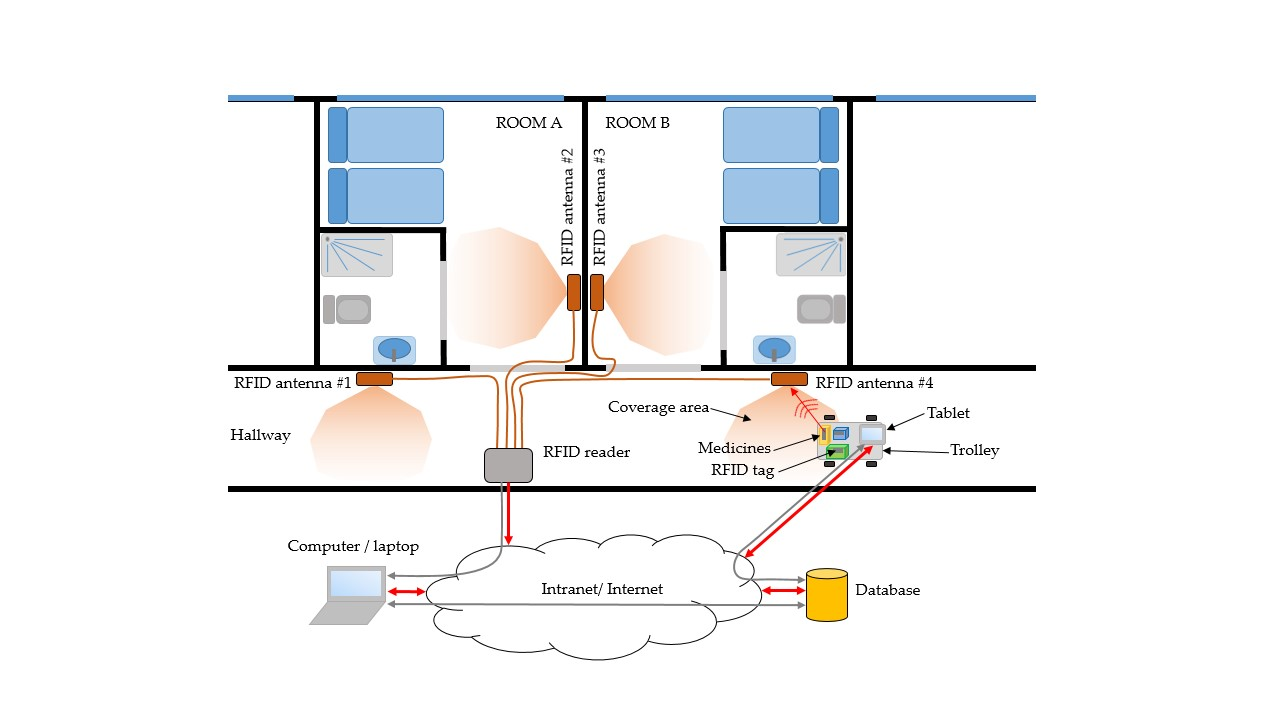
\includegraphics[width=\textwidth]{app_functionality} 
\caption{\label{fig:appfunctionality}Application scenario of RFID application } 
\end{figure}

\subsection{Possibilities of extension}

Henrici \cite[p.121 ff.]{henrici} describes four alternative channels to authenticate and authorized the right tags and to prevent attacks on RFID applications. 
The first possibility of an alternative channel is to use written text to authenticate special operations, for instance on packaging. The master key can be printed on the interior of the product package and is proposed as key recovery mechanism.
Furthermore, optical barcodes can be used together with RFID to ensure identification of items. Especially barcodes attached to each item can be used for general identification of objects. Additionally, RFID tags might be used to assign items of high value.
A third possibility of using side channels is to use optical input, such as photodiodes attached to RFID tags. Each RFID tag can use flashes of light (also called optical channel) to transfer data.   
Lastly, a physical contact channel can also be used alternatively. Compared to smartcards, this methods defends against wireless sabotage or denial of service attacks.


















 
